\documentclass[10pt,twocolumn,letterpaper]{article}

\usepackage{cvpr}
\usepackage{times}
\usepackage{epsfig}
\usepackage{graphicx}
\usepackage{amsmath}
\usepackage{amssymb}
\usepackage{gensymb}
\usepackage{url}

% Include other packages here, before hyperref.

% If you comment hyperref and then uncomment it, you should delete
% egpaper.aux before re-running latex.  (Or just hit 'q' on the first latex
% run, let it finish, and you should be clear).
%\usepackage[pagebackref=true,breaklinks=true,letterpaper=true,colorlinks,bookmarks=false]{hyperref}

\cvprfinalcopy % *** Uncomment this line for the final submission

\def\cvprPaperID{****} % *** Enter the 3DV Paper ID here
\def\httilde{\mbox{\tt\raisebox{-.5ex}{\symbol{126}}}}

% Pages are numbered in submission mode, and unnumbered in camera-ready
%\ifcvprfinal\pagestyle{empty}\fi
\setcounter{page}{1}
\begin{document}

%%%%%%%%% TITLE
\title{Omni-directional stereo for 360$\degree$ 3D virual reality video}

\author{Prashanth Chandran\\
ETH Zurich\\
www.ethz.ch\\
{\tt\small chandranp@student.ethz.ch}
% For a paper whose authors are all at the same institution,
% omit the following lines up until the closing ``}''.
% Additional authors and addresses can be added with ``\and'',
% just like the second author.
% To save space, use either the email address or home page, not both
\and
Sasha Pagani\\
ETH Zurich\\
www.ethz.ch\\
{\tt\small paganis@student.ethz.ch}
\and
Julia Giger\\
ETH Zurich\\
www.ethz.ch\\
{\tt\small jgiger@student.ethz.ch}
}

\maketitle
%\thispagestyle{empty}

%%%%%%%%% ABSTRACT
\begin{abstract}
   This project is an implementation of an Omni directional stereo (ODS) renderer; 'Jump', that was proposed by Anderson et.al in \cite{jump16}.  To render ODS content, we worked with data that was captured from a camera rig consisting of 10 cameras. The ODS rendering pipeline proposed by  \cite{jump16} consists of the stages of camera calibration, optical flow estimation, exposure correction, view interpolation, and composting. Staying mostly faithful to the rendering pipeline of \cite{jump16}, we introduced a few simplifications owning to the limitations of our camera rig and time considerations. The renderer was implemented from scratch in Python and relies on OpenCV only for image I/O and optical flow calculation. Our ODS renderer is extremely generic, easy to use and can be readily used to render ODS content from an arbitrary rig only given its calibration data. 
\end{abstract}

%%%%%%%%% BODY TEXT
\section{Introduction}

An ideal virtual reality environment is one where the user can experience the world in 1) stereo, where eye get an image appropriate to where the user is sees, and 2) in 360 degrees, where the user is free to look in any direction. The rendering of Omni directional stereo content is therefore absolutely necessary for visual immersion. 

The primary reason why VR environments have to be rendered in stereo is because of the way in which humans perceive depth. The perception of depth in human stereo or binocular vision is a result of the fusion of images captured by the left and right eyes. 
In order to render stereo images, we need to capture synchronized frames from two cameras set apart by the interpupillary distance (IPD); which denotes the distance between our two eyes. The IPD on average about 6.4 cm. However, since for applications in virtual reality, we not only require images that are rendered in stereo, but for them to also be omni-directional. 

One straight forward method of capturing such videos in 360 would be to use two omni-directional cameras that are separated by the human IPD. This method however, suffers from two limitations. The first problem with such an approach is that the two cameras would see each other. The second and more important problem is that the objects which lie on the line passing through the two camera centers will have no disparity (see figure~\ref{two_360}). The absence of disparity makes the perception of depth impossible and therefore, with this simple solution, we would not be able to render  videos in omni-directional stereo.

Ideally, what we want is to have a stereo image pair for every orientation of the head (see figure~\ref{wanted}). This would result in the capture of a huge number of images. Instead, if we could capture only the central ray from each camera and borrow other rays from the central rays of neighbouring camera positions, we could greatly reduce the number of images we need(see figure~\ref{approx}). Figure~\ref{ods} illustrates the extension of this approach to 360$\degree$.

This report is organized as follows. In section \ref{related-work}, we discuss related work and highlight the contributions of \cite{jump16}. Section \ref{work-division} describes how the work was split among the members of our team. Section \ref{method} describes our implementation of the ODS stitching pipeline in detail. In section \ref{resultsdis}, we present the results obtained using our renderer and discuss its advantages and shortcomings. Our contributions are summarized in section \ref{conclusion}.

\begin{figure}[t]
\begin{center}
   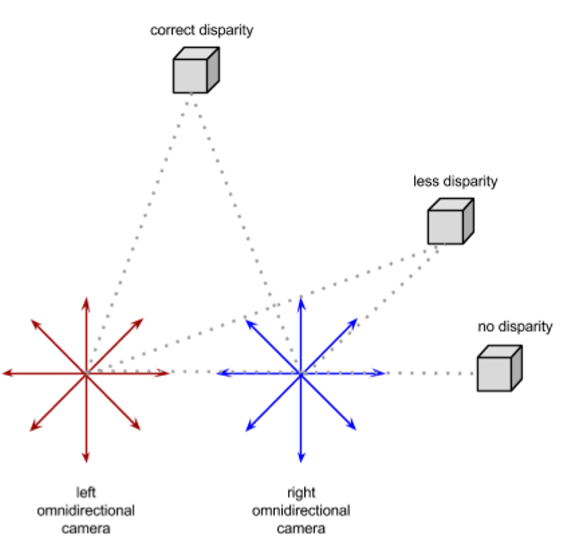
\includegraphics[width=0.8\linewidth]{pictures/two_360.png}
\end{center}
   \caption{Illustration of two 360$\degree$ cameras placed next to each other. This figure has been borrowed from \cite{ods}.}
\label{two_360}
\end{figure}

\begin{figure}[t]
\begin{center}
   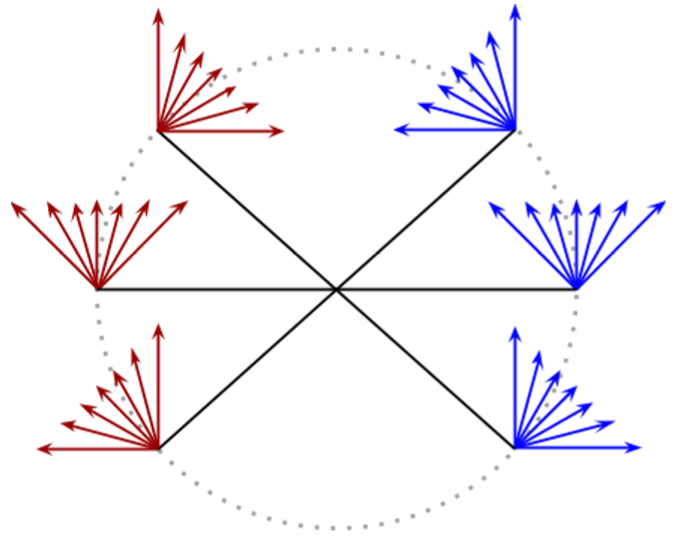
\includegraphics[width=0.5\linewidth]{pictures/wanted.png}
\end{center}
   \caption{This image depicts the optimal situation, where a full image is captured for each orientation of head and for each eye. The red rays illustrate the left eye and the blue ones the left eye. This figure has been borrowed from \cite{ods}.}
\label{wanted}
\end{figure}

\begin{figure}[t]
\begin{center}
	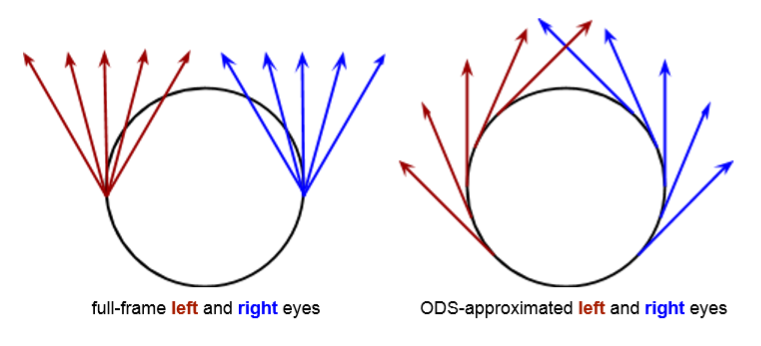
\includegraphics[width=0.8\linewidth]{pictures/approxi.png}
\end{center}
   \caption{The image on the left shows represents viewing rays for each eye when the entire image is captured for each viewing direction. The image on the right illustrates the ODS approximation of the left image, where in only the central ray for each camera position is captured. This figure has been borrowed from \cite{ods}.}
\label{approx}
\end{figure}

\begin{figure}[t]
\begin{center}
   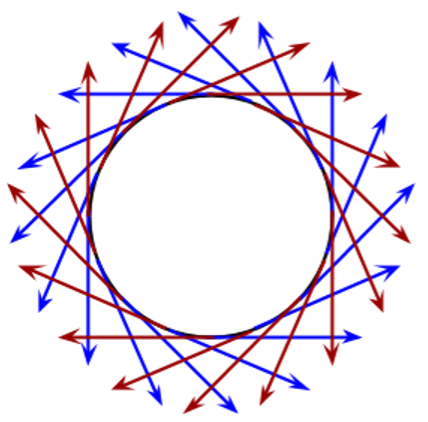
\includegraphics[width=0.5\linewidth]{pictures/ods.png}
\end{center}
   \caption{This image shows the viewing ray directions (per eye) when the ODS approximation is done for 360$\degree$. The red rays correspond to the left eye and the blue ones to the right eye. This figure has been borrowed from \cite{ods}.}
\label{ods}
\end{figure}


%------------------------------------------------------------------------
\section{Related work}
\label{related-work}
Several methods in the past have been proposed to tackle the problem of rendering omni directional stereo content. We discuss two such methods that are particularly interesting. 'Omnistereo: Panaromic stereo imaging', proposed in \cite{peleg}, described the multiple view point projection involved in the generation of omni-directional stereo images. The authors used a single rotating camera to capture images in 360 degrees. Another approach is 'MegaStereo' \cite{megastereo}. 

Both methods \cite{peleg} and \cite{megastereo}, capture omni-directional panaromas with a single rotating camera. This means that they rely on the scene being static or that there is little motion. In \cite{jump16}, the authors propose a new camera rig with 16 cameras that allows for large scene motion. They also use optical flow based view interpolation to synthesize images between adjacent cameras in the rig. A key contribution of \cite{jump16} is that their view interpolation and composting framework, can generate ODS panaromas from only 16 images, while previous methods like \cite{megastereo} required hundreds of images. 

\subsection{Our implementation of \textit{Jump} \cite{jump16}}
In this project, our goal was to implement the ODS stitching pipeline proposed by Anderson et al.~\cite{jump16}. While staying loyal to main steps of their stitching pipeline, we would like to highlight a few differences in our implementation. 

The first difference is that we did not have access to the 'Go-Pro Oddessy' rig that was designed and used by the authors of \cite{jump16} to capture 360 degree content. Instead, we were provided with a dataset that was recorded from a rig of 10 cameras. More details about the deviations of this camera rig from the one used in \cite{jump16} are provided in section \ref{sec:camera-rig}. 

The second is that the authors in \cite{jump16}, proposed a novel optical flow algorithm, that was designed to be optimal for the task of view interpolation in scenes with large motion.  Owing to time constraints, we do not implement the optical flow they propose and instead use an off the shelf dense optical algorithm. 

Furthermore, we had to simplify the final composting step because we did not have as many images to blend as in \cite{jump16}.

%------------------------------------------------------------------------
\section{Work subdivision}
\label{work-division}
The steps involved in our ODS stitching pipeline is shown in figure \ref{pipeline}. Work was divided among our team members as follows. 
\begin{itemize}
\item \textbf{Prashanth Chandran}
\begin{itemize}
\item View interpolation and ODS stitching
\item Experiments with homography based stitching and other visualizations
\item Exposure correction
\item Final report
\end{itemize}
\item \textbf{Sasha Pagani}
\begin{itemize}
\item Optical flow estimation with openCV
\item Camera calibration
\item Experiments with Unity on the Google cardboard
\item Mid-term review presentation
\item Final report
\end{itemize}
\item \textbf{Julia Giger}
\begin{itemize}
\item View interpolation and ODS stitching
\item Experiments with Unity on the Google cardboard
\item Mid-term review presentation
\item Final report
\end{itemize}
\end{itemize}

%------------------------------------------------------------------------
\section{Method}
\label{method}
As mentioned before, figure~\ref{pipeline} depicts our ODS stitching pipeline. The inputs to our renderer are synchronized videos captured from 10 cameras arranged on a rig. As a first step, these cameras are calibrated to scale using standard structure from motion algorithms \cite{sfm}. For synthesizing novel views between adjacent cameras, dense optical flow is estimated between temporally consistent frames of neighbouring camera pairs. Camera gains that compensate for differences in camera exposure are then calculated in an exposure correction step. Using the previously estimated optical flow, a novel linear view interpolation, as proposed by \cite{jump16} is carried out and the images are composted to result in an ODS panaroma.  
\begin{figure}[t]
\begin{center}
   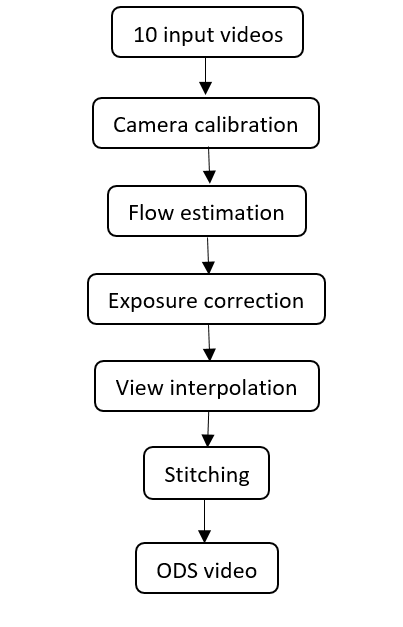
\includegraphics[width=0.5\linewidth]{pictures/pipeline.PNG}
\end{center}
   \caption{ODS rendering pipeline. }
\label{pipeline}
\end{figure}

\subsection{Camera rig and calibration}
\label{sec:camera-rig}
The 10 cameras in the rig were calibrated with the help of 'Kalibr' \cite{kalibr}. The calibration data consists of the intrinsics and the relative extrinsics of each camera. For our rendering purposes, we would need the global extrinsics (the extrinsics of each camera with respect to the origin), as opposed to the relative extrinsics (which is w.r.t location and orientation of the previous camera in the rig). Global extrinsics for each camera was calculated from the relative extrinsics using equation \ref{eq:extrinsics}. 
\begin{equation}
GE_i = GE_{i-1} \cdot RE_{i}^{-1}
\label{eq:extrinsics}
\end{equation}
where $GE_i$ represents global extrinsics (w.r.t to the origin) of camera i while $RE_i$ represents the relative extrinsics (with respect to the previous camera) of camera i. Camera 0 was assumed to be at the origin.

Figure \ref{fig:rig} shows how the cameras in our rig are arranged. The circle in red is the viewing circle: i.e. the circle from which the ODS viewing rays emanate. The projections of the camera centres for each eye onto the viewing circle are also shown in figure \ref{fig:rig}. 

\begin{figure}[t]
\begin{center}
   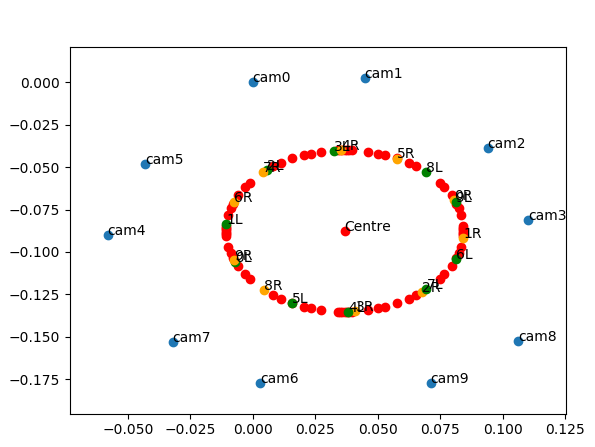
\includegraphics[width=0.8\linewidth]{pictures/our_camera_rig.PNG}
\end{center}
   \caption{An illustration of the arrangement of cameras on the rig, the viewing circle and the projection of the camera centres onto the viewing circle for the left and right eyes. The points in green on the viewing circle are camera centre projections computed for the left eye and those in orange correspond to the projections for the right eye.}
\label{fig:rig}
\end{figure}

Figure \ref{fig:imageplanes} displays the image planes captured by each camera in the rig. As one can see, the rig is composed of 5 pairs of stereo cameras. There is a strong overlap in the images captured by a stereo pair and very less overlap between the images captured by two different stereo pairs. For example, there is very good overlap between the images captured by cameras 0 and 1, while there is very little overlap between the images of cameras 1 and 2. 
\begin{figure}[t]
\begin{center}
   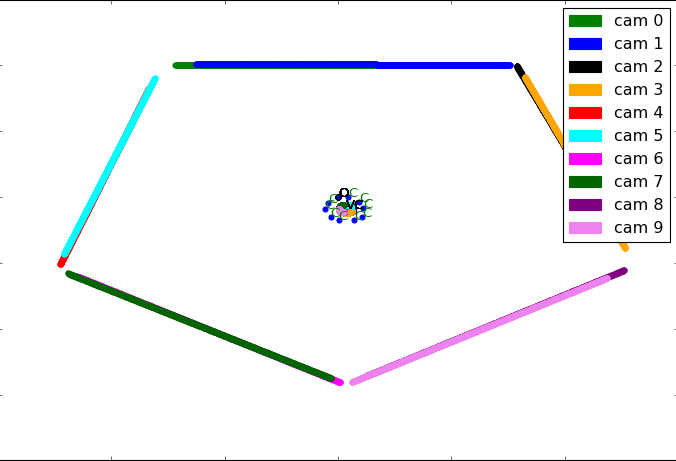
\includegraphics[width=0.7\linewidth]{pictures/rig_detailed.png}
\end{center}
   \caption{Visualizing the image planes as captured by our camera rig.}
\label{fig:imageplanes}
\end{figure}

\subsection{Flow estimation}
\label{sec:flow}
When optical flow is computed between temporally consistent frames of a two spatially separated cameras, the horizontal flow approximates disparity. To compute per-pixel optical flow vectors, we use the two frame optical flow estimation algorithm that was proposed by \cite{farneback}. Figure \ref{fig:optical-flow-01} shows the result of our dense optical flow estimation. In figure \ref{fig:optical-flow-01}, optical flow was estimated between two corresponding frames of cameras 0 and 1. 
\begin{figure}
\centering
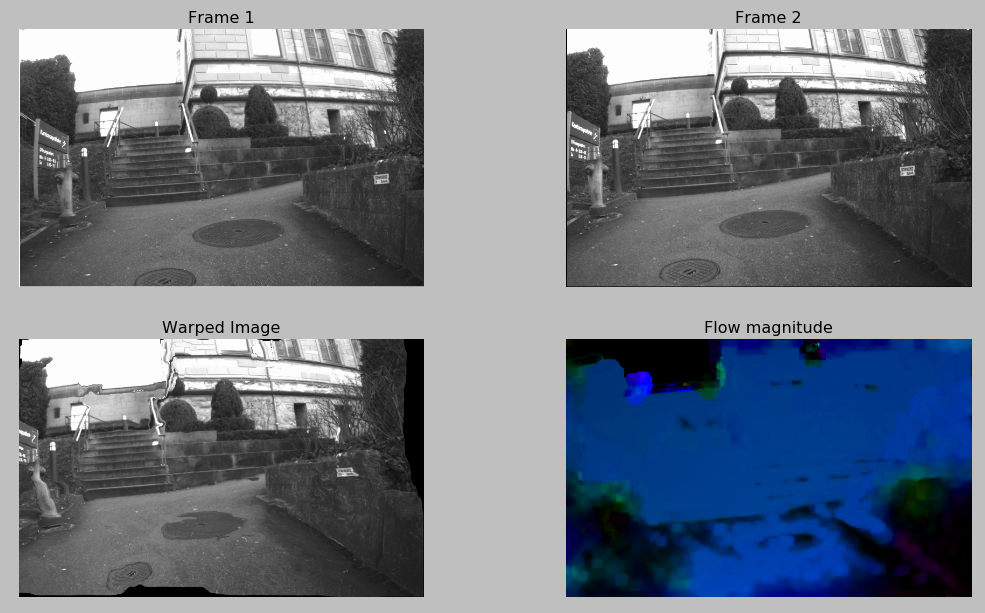
\includegraphics[width=\linewidth]{../results/optical-flow/cam0-cam1-proper.png}
\caption{\textit{Top left}:  Image captured by camera 0. \textit{Top right}: Image captured by camera 1. \textit{Bottom left}: The image captured by camera 0 has been warped according to the estimated flow. We see that image has rightly been displaced to the left. \textit{Bottom right}: Horizontal flow vectors visualized in HSV color space.}
\label{fig:optical-flow-01}
\end{figure}

Note that this method of estimating optical flow between two cameras works well only when there is sufficient overlap between the two cameras. When the motion between two neighbouring cameras is large; as is the case between two neighbouring stereo pairs in our rig: for example cameras 1 and 2, the optical flow estimate goes wrong. We discuss these effects in detail in section \ref{resultsdis}.

\subsection{Exposure correction}
We implemented the exposure correction algorithm from \cite{jump16}. First, the region of overlap between every pair of neighbouring images is identified. This is done by detecting correspondences between the two images. The average intensity in the region of overlap of an image with its previous and next image in the camera rig are calculated. Let these intensities be denoted by $P_i$ and $N_i$ respectively. We estimate the gain to be applied to each image $g_i$, by minimizing 
\begin{equation}
\sum_{i=1}^{n}(g_{i}N_{i} - g_{i+i}P_{i+i})^2 + \epsilon(1-g_{i})^2
\label{eq:gain1}
\end{equation}
The second term in equation \ref{eq:gain1} corresponds to a prior which requires gains to be close to 1. Once the gains $g_i$'s have been calculated for each image, the gain for each column is computed as a weighted average of gains computed for neighbouring cameras. 
\begin{equation}
g_{c}=\dfrac{(\theta_{c}-\theta_{0})}{(\theta_1-\theta_{0})}*g_{0} + \dfrac{(\theta_{1}-\theta_{c})}{(\theta_1-\theta_{0})}*g_{1}
\label{eq:gain2}
\end{equation}
In eq. \ref{eq:gain2}, $\theta_0$ and $\theta_1$ correspond to locations where two cameras on either side of column 'c' map onto the ODS panaroma. $\theta_c$ is the location where column 'c' maps onto the ODS panaroma.

\subsection{View interpolation}
\label{sec:viewinterp}
To synthesize views between two neighbouring cameras, we use the linear view interpolation algorithm (eq. \ref{eq:interp}) as proposed  in \cite{jump16}.
\begin{equation}
\theta_p=\dfrac{(\theta_{b}-\theta_{1})*\theta_{0}+(\theta_{0}-\theta_{a})*\theta_{1}}{\theta_{b}-\theta_{a}+\theta_{0}-\theta_{1}}
\label{eq:interp}
\end{equation}
where $\theta_{0}$ and $\theta_ {1}$ are the headings of the two cameras in the ODS stitch. $\theta_ {a}$ is the heading of a point in the first camera and $\theta_ {b}$ is the heading of the same point; as calculated by optical flow, in the second camera. These angles are illustrated in figure \ref{fig:interpolation}.

\begin{figure}[t]
\begin{center}
   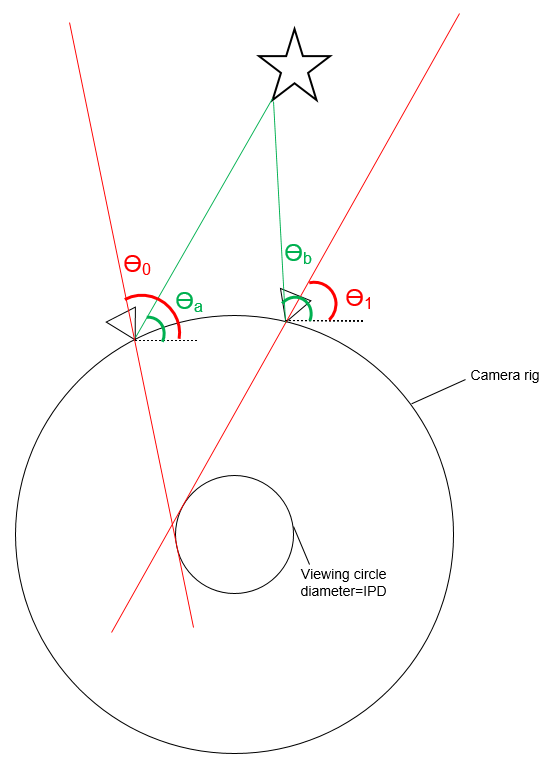
\includegraphics[width=0.7\linewidth]{pictures/interpolation.PNG}
\end{center}
   \caption{An illustration of the different angles used in the view interpolation formula. The red lines are the central rays of two cameras between which a novel view is being synthesized. The green lines are rays corresponding to the same point as seen from two different cameras.}
\label{fig:interpolation}
\end{figure}

\subsection{Stitching}
Once novel views have been synthesized between cameras, they are projected onto the ODS stitch as explained in section \ref{sec:viewinterp}. We use a simple weighted average to blend the images on the final ODS panaroma. Using more sophisticated algorithms for blending will of course yield better results. 
%------------------------------------------------------------------------
\section{Results and Discussion}
\label{resultsdis}
For testing our implementation we used a dataset that was provided by our supervisor. 
\subsection{Optical flow for dense correspondences}
\label{sec:challenges-flow}
As discussed in section \ref{sec:flow}, estimating optical flow between two cameras with \cite{farneback} works satisfactorily when the motion between the two cameras is small. In figure \ref{fig:optical-flow-45}, we see the result of estimating optical flow between cameras 4 and 5. 
\begin{figure}
\centering
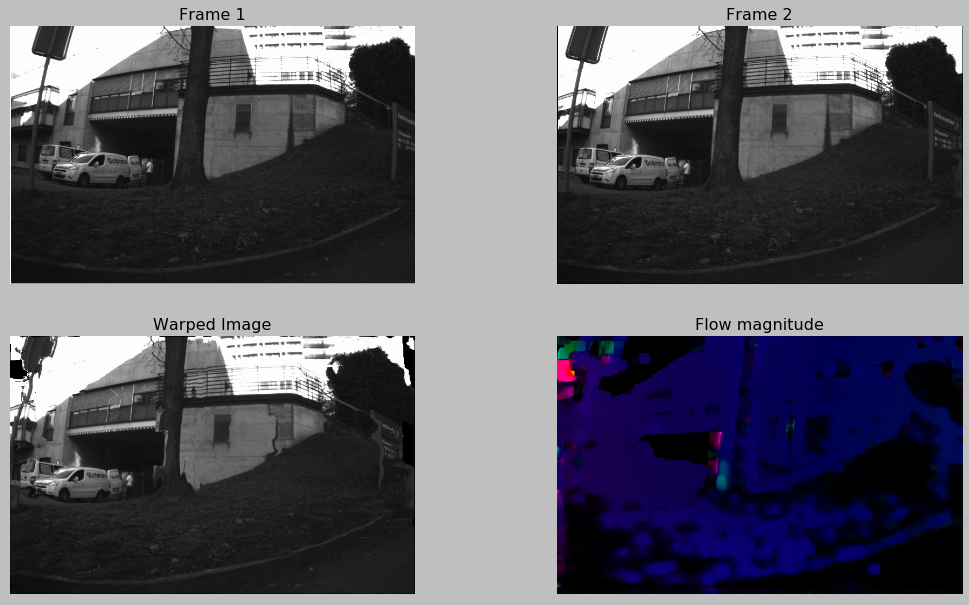
\includegraphics[width=\linewidth]{../results/optical-flow/cam4-cam5-proper.png}
\caption{\textit{Top left}:  Image captured by camera 4. \textit{Top right}: Image captured by camera 5. \textit{Bottom left}: The image captured by camera 4 has been warped according to the estimated flow. We see that image has rightly been displaced to the left. \textit{Bottom right}: Horizontal flow vectors visualized in HSV color space.}
\label{fig:optical-flow-45}
\end{figure}

However, when we attempt to compute optical flow between images where there is very little overlap: for example the images captured by camera 1 and camera 2 where the two images look quite different from each other; the optical flow estimate is incorrect. This is as shown in the figure \ref{fig:optical-flow-74}.

\begin{figure}
\centering
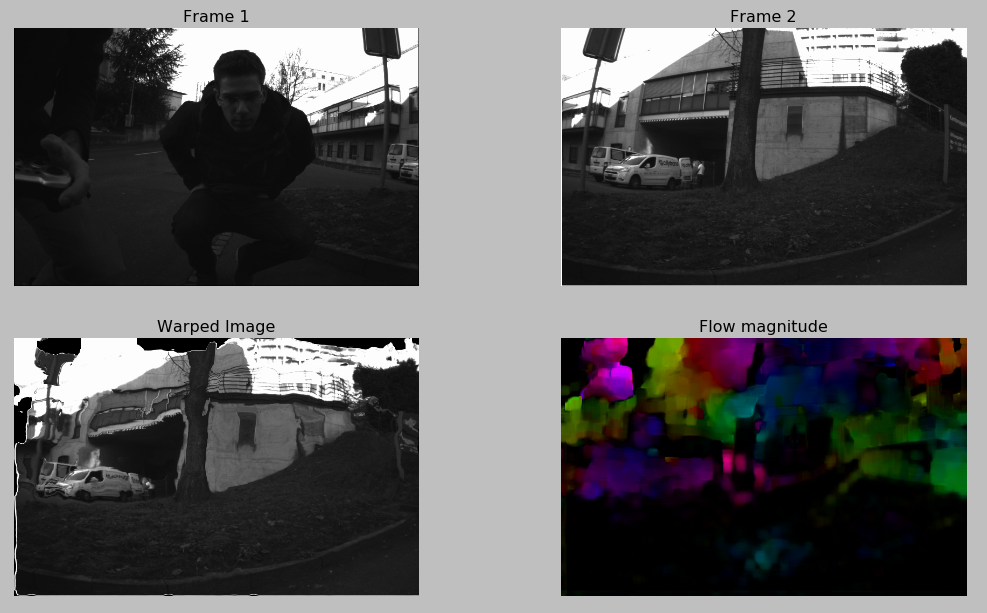
\includegraphics[width=\linewidth]{../results/optical-flow/cam7-cam4-bad.png}
\caption{\textit{Top left}:  Image captured by camera 7. \textit{Top right}: Image captured by camera 4. \textit{Bottom left}: The image captured by camera 4 has been warped according to the estimated flow. \emph{The flow vectors are incorrect in this case as is seen from the result of the warp. Ideally, image on the right (from camera 4) has to be displaced to the extreme right in the warped image to correspond with the capture from camera 7.} \textit{Bottom right}: Horizontal flow vectors visualized in HSV color space.}
\label{fig:optical-flow-74}
\end{figure}

For obtaining correspondences between such wide baseline images, we tried to use standard feature matching techniques such as SIFT \cite{sift}. We found feature matching with SIFT to be much better at finding correspondences in scenes with large motion than the flow based technique used in \cite{jump16}. Figure \

\begin{figure}
\centering
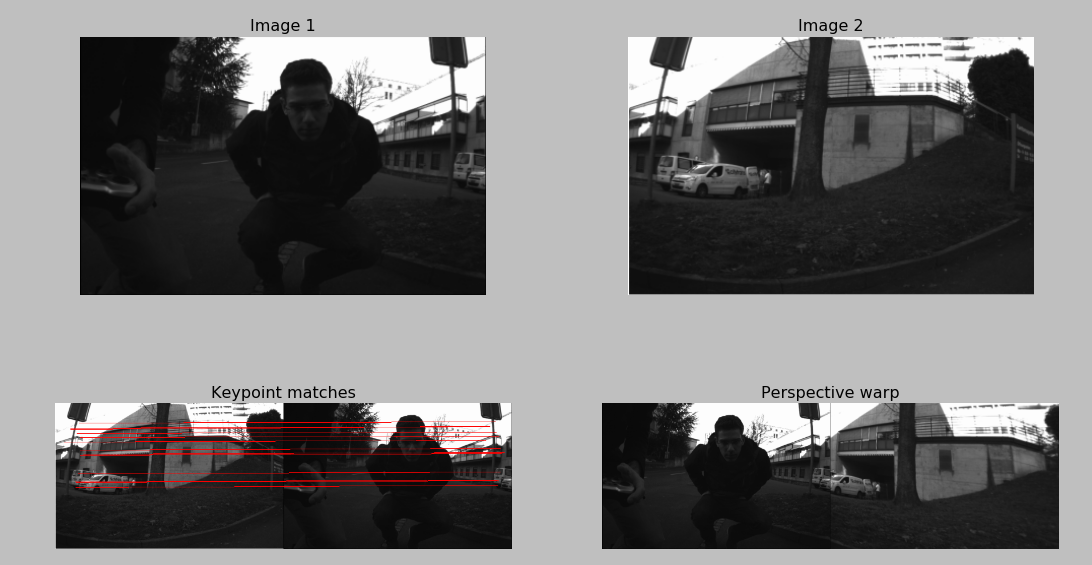
\includegraphics[width=\linewidth]{../results/homography-stitch/cam7-cam4-good.png}
\caption{Homography based stitching of two images with SIFT. Top left: Image captured from camera 7. Top right: Image captured from camera 4. Bottom left: Key point matches. Bottom right: The image from camera 7 has been perspective warped onto the image plane of camera 4. In this case, we see that because the key point matches are accurate, we get a good stitch.}
\label{fig:homo-74}
\end{figure}

Unfortunately, the overlap between certain cameras in our rig is so small that even wide baseline feature matching techniques don't work all the time. This is illustrated in figure \ref{fig:homo-12}.
\begin{figure}
\centering
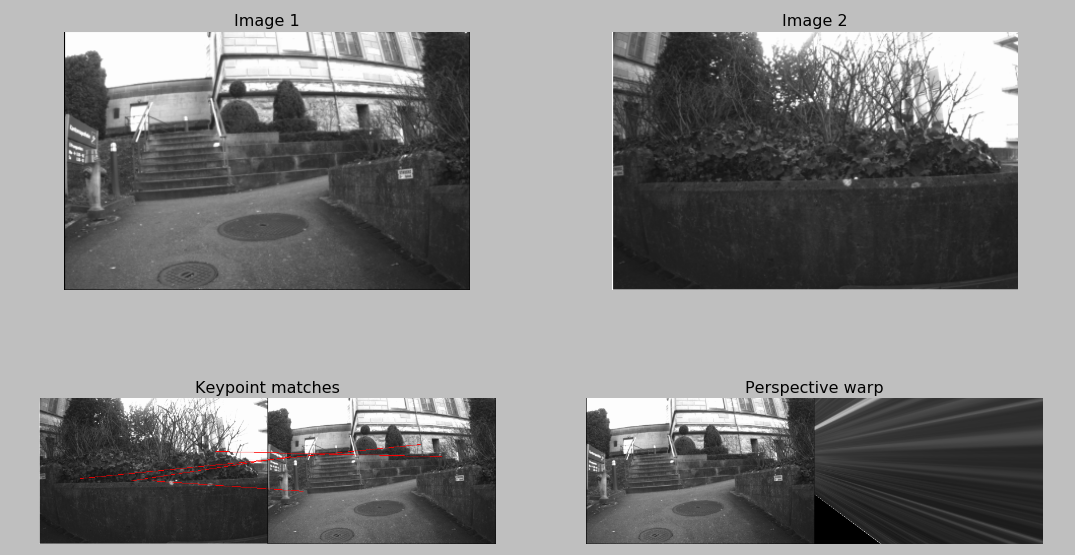
\includegraphics[width=\linewidth]{../results/homography-stitch/cam1-cam2-bad.png}
\caption{SIFT correspondences between images captured by camera 1 and camera 2. Even SIFT feature matching fails in this case and we get a very distorted homography stitch.}
\label{fig:homo-12}
\end{figure}

Finding dense correspondences between neighbouring images is vital to being able to synthesize novel views between cameras. The interpolation in equation \ref{eq:interp}, relies heavily on the fact that we have reliable correspondences for every pixel in an image. 
Given the problems discussed herein; using optical flow to synthesize views between two stereo camera pairs such as cam0-cam1 and cam2-cam3 etc isn't possible. 

Using optical flow to find dense correspondences between cameras is not a problem for the authors in \cite{jump16} because of the fact that there is sufficient overlap between images captured by two neighbouring cameras on their camera rig. Also, all cameras in their rig are oriented radially outwards as opposed to the stereopairs in our rig. Furthermore, they also use a more sophisticated algorithm for computing dense flow which is capable of handling large motion.

\subsection{Content rendered by our ODS renderer}
\label{ods-results}
We refer the reader to figure \ref{fig:imageplanes} to note that the cameras in our rig are numbered as follows: starting clockwise (0, 1, 2, 3, 8, 9, 6, 7, 4, 5). Following the problems mentioned in section \ref{sec:challenges-flow}, we were able to interpolate views only between cameras (0-1, 2-3, 8-9 etc) and not between adjacent stereo cameras pairs i.e. between cameras 1-2, 3-8 etc. As a result, black stripes in the ODS panaroma are to be expected. 

Figures  ~\ref{fig:lefteye_pwise} and ~\ref{fig:lefteye_cwise} show two variations of the 360 degree ODS stitch produced by our renderer for the left eye. In figure \ref{fig:lefteye_pwise}, we use every pixel's horizontal flow vector in determining it's position in the ODS panaroma according to eq. \ref{eq:interp}. In figure \ref{fig:lefteye_cwise}, we only consider the average horizontal flow of every column in the image to determine the column's final position in the ODS stitch. This results in significantly faster rendering as one would expect. 

A careful reader must have observed that the second image stripe from left in figures \ref{fig:lefteye_cwise} and \ref{fig:lefteye_pwise} seem abnormal. This is because one of the cameras in the rig viz. camera 3, was not functioning as expected. Therefore the images captured by it seem abnormal. These are not artefacts produced during rendering. 
 
\begin{figure}[t]
\begin{center}
   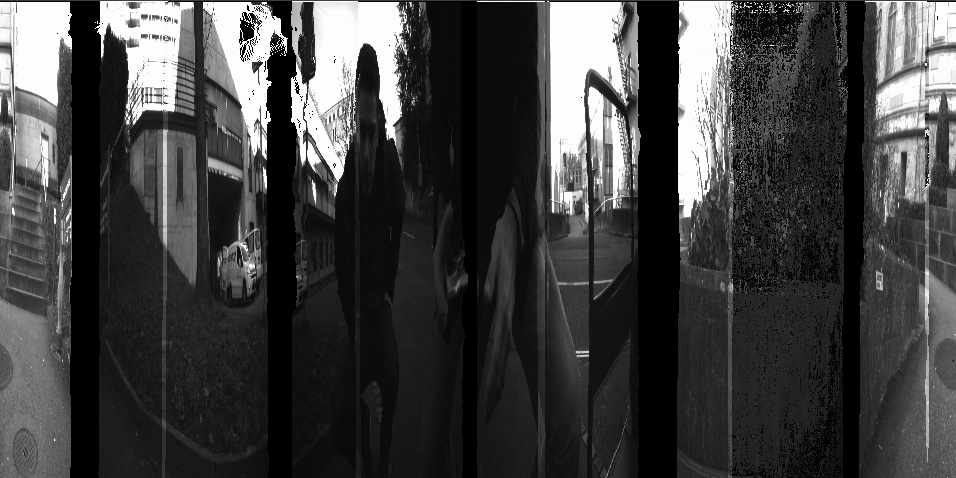
\includegraphics[width=\linewidth]{../results/ODS-renderer-results/frame0_lefteye_pwise.png}
\end{center}
   \caption{ODS stitch result for the left eye with pixel wise flow for view interpolation.}
\label{fig:lefteye_pwise}
\end{figure}

\begin{figure}[t]
\begin{center}
   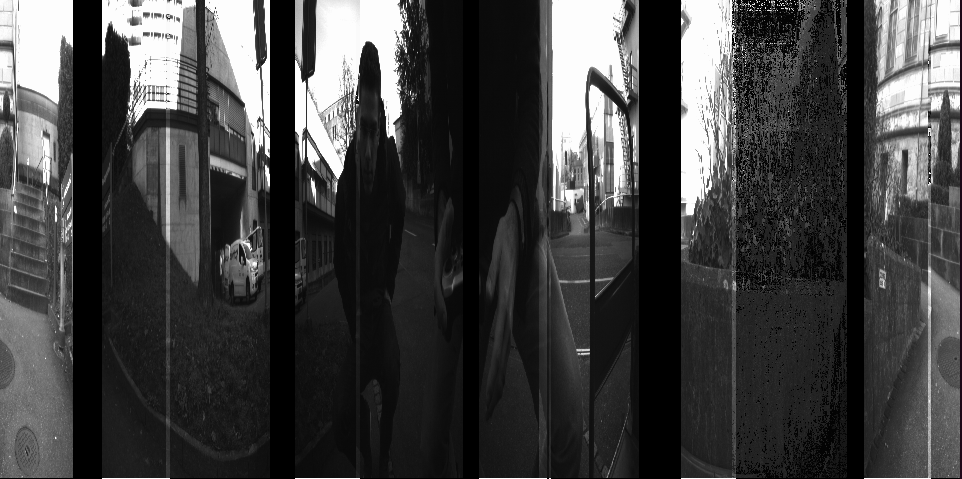
\includegraphics[width=\linewidth]{../results/ODS-renderer-results/frame0_lefteye_cwise.png}
\end{center}
   \caption{ODS stitch result for the left eye with column wise flow for view interpolation.}
\label{fig:lefteye_cwise}
\end{figure}

ODS content for viewing in a VR device such as the Google cardboard is generally rendered as two images stacked on top of each other.  With the given dataset and our rendering pipeline, we were able to generate the result shown in figure \ref{fig:left_right_eyecwise}.
\begin{figure}
\centering
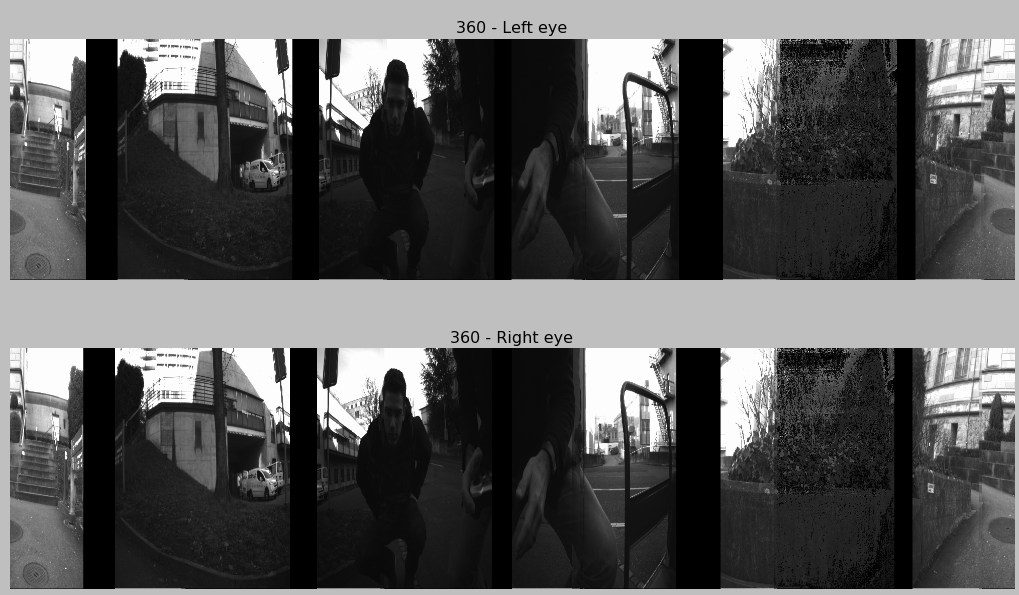
\includegraphics[width=\linewidth]{../results/ODS-renderer-results/left-right-eye.png}
\caption{Rendered ODS images for the left and right eye.}
\label{fig:left_right_eyecwise}
\end{figure}

\subsection{Implementation details}
\begin{itemize}
\item Our ODS renderer was written from scratch in Python. All of the multiview projection geometry was implemented. Our renderer relies on OpenCV only for Image I/O operations and for computing the optical flow. 
\item Given a .yaml camera calibration file, our renderer can be extended to any arbitrary camera rig without any modification. This highlights the generic nature of our implementation. 
\item Our implementation takes approximately 6 seconds to render a 2K panaroma when column wise flow for interpolation is used. It takes about 2 minutes to render a 2K panaroma when per-pixel flow for interpolation is used. 
\item Though exposure correction has been implemented and tested (refer file \emph{ExposureCorrect.py} in the handout), we weren't able to use it in the final ODS rendering results because of black stripes in the rendered results. 
\end{itemize}
%------------------------------------------------------------------------
\section{Conclusion}
\label{conclusion}
In this project, we implemented an ODS renderer based on \cite{jump16} that can render 360 stereo video.  The results obtained by Anderson et al.~\cite{jump16} are much better than ours but this was to be expected for several reasons. Firstly, the authors in \cite{jump16} designed and used a perfectly radial Odyssey GoPro rig with 16 cameras. Results in this project, on the other hand are rendered from only different 10 cameras with a different rig geometry. We also use an off the shelf optical flow algorithm instead of the much more powerful optical flow algorithm proposed in \cite{jump16}. Our composting methods are much simpler than those used in \cite{jump16} too. With improvements to the optical flow and compositing algorithms, and with a camera rig similar to that used in \cite{jump16}, we are confident that our renderer will produce better results.

{\small
\bibliographystyle{ieee}
\bibliography{egbib}
}

\end{document}
